\documentclass[12pt]{article}

% Imports
\usepackage{hyperref}
\usepackage[margin=0.5in]{geometry}
\usepackage{ctable}
\usepackage{array}
\usepackage{graphicx}
\usepackage{fancyvrb}
\usepackage{titlesec}

% Paragraph spacing
\setlength{\parindent}{0em}
\setlength{\parskip}{0.5em}

% Default font
\renewcommand*{\familydefault}{\sfdefault}

% title spacing
\titlespacing*{\section}
{0pt}{2pt}{0pt}
\titlespacing*{\subsection}
{0pt}{2pt}{0pt}

% table lines
\newcolumntype{?}{!{\vrule width 1pt}}

% hyperlinks
\hypersetup{
  breaklinks=true,  % so long urls are correctly broken across lines
  colorlinks=true,
  urlcolor=blue,
  linkcolor=red,
  citecolor=red,
 }

\begin{document}

% Header info
\textbf{CSE 291 - PERSONAL GENOMICS FOR BIOINFORMATICIANS}

\section*{Problem Set 1 - Introduction to human genomes}

This homework should be sent to mgymrek@ucsd.edu with subject line \textcolor{purple}{[CSE291 PS1:LASTNAME]} by the beginning of class on \textbf{Thursday, January 12}. The assignment is worth 5 points total.

\subsection*{Objectives}
\begin{itemize}
\setlength\itemsep{0.0em}
\item Review human genetics concepts.
\item Get comfortable using the SDSC cluster and with standard file formats and tools for analyzing genomes.
\end{itemize}

\subsection*{Exercises}
\begin{enumerate}
\setlength\itemsep{0.0em}

\item \textbf{(0.25 points)} How many chromosomes does a typical human have?

\item \textbf{(0.25 points)} Approximately what percent of the genome consists of protein coding genes?

\item \textbf{(0.25 points)} Identify the labeled components of a typical gene depicted below. Options are: exon, intron, 5'UTR, 3'UTR, splice site, promoter/regulatory region.
\begin{figure}[h!]
\centering
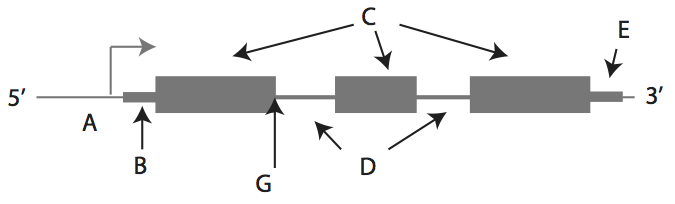
\includegraphics[width=200px]{pset1gene.png}
\end{figure}

\item \textbf{(0.25 points)} You see a gene with the following coding sequence: ATGCCGAATCGATCGTAA. Give (1) the sequence of the transcribed mRNA and (2) the amino acid sequence of the translated protein.
% Met P N R S Stop

\item \textbf{(0.25 points)} A mutation occurs in the gene from the previous question, resulting in a sequence ATGCCGAATCGATCTTAA. What is the amino acid sequence now? This is known as a \emph{synonymous mutation}.
% Met P N R S Stop

\item \textbf{(0.25 points)} A different mutation occurs in the same gene, now resulting in a sequence ATGCCGAATCGACCGTAA. What is the amino acid sequence of the new protein? This is known as a \emph{missense mutation}.
% Met P N R P Stop

\item \textbf{(0.25 points)} What modes of inheritance are consistent with the following pedigree? Name an example human condition that follows this mode of inheritance.
\begin{figure}[h!]
\centering
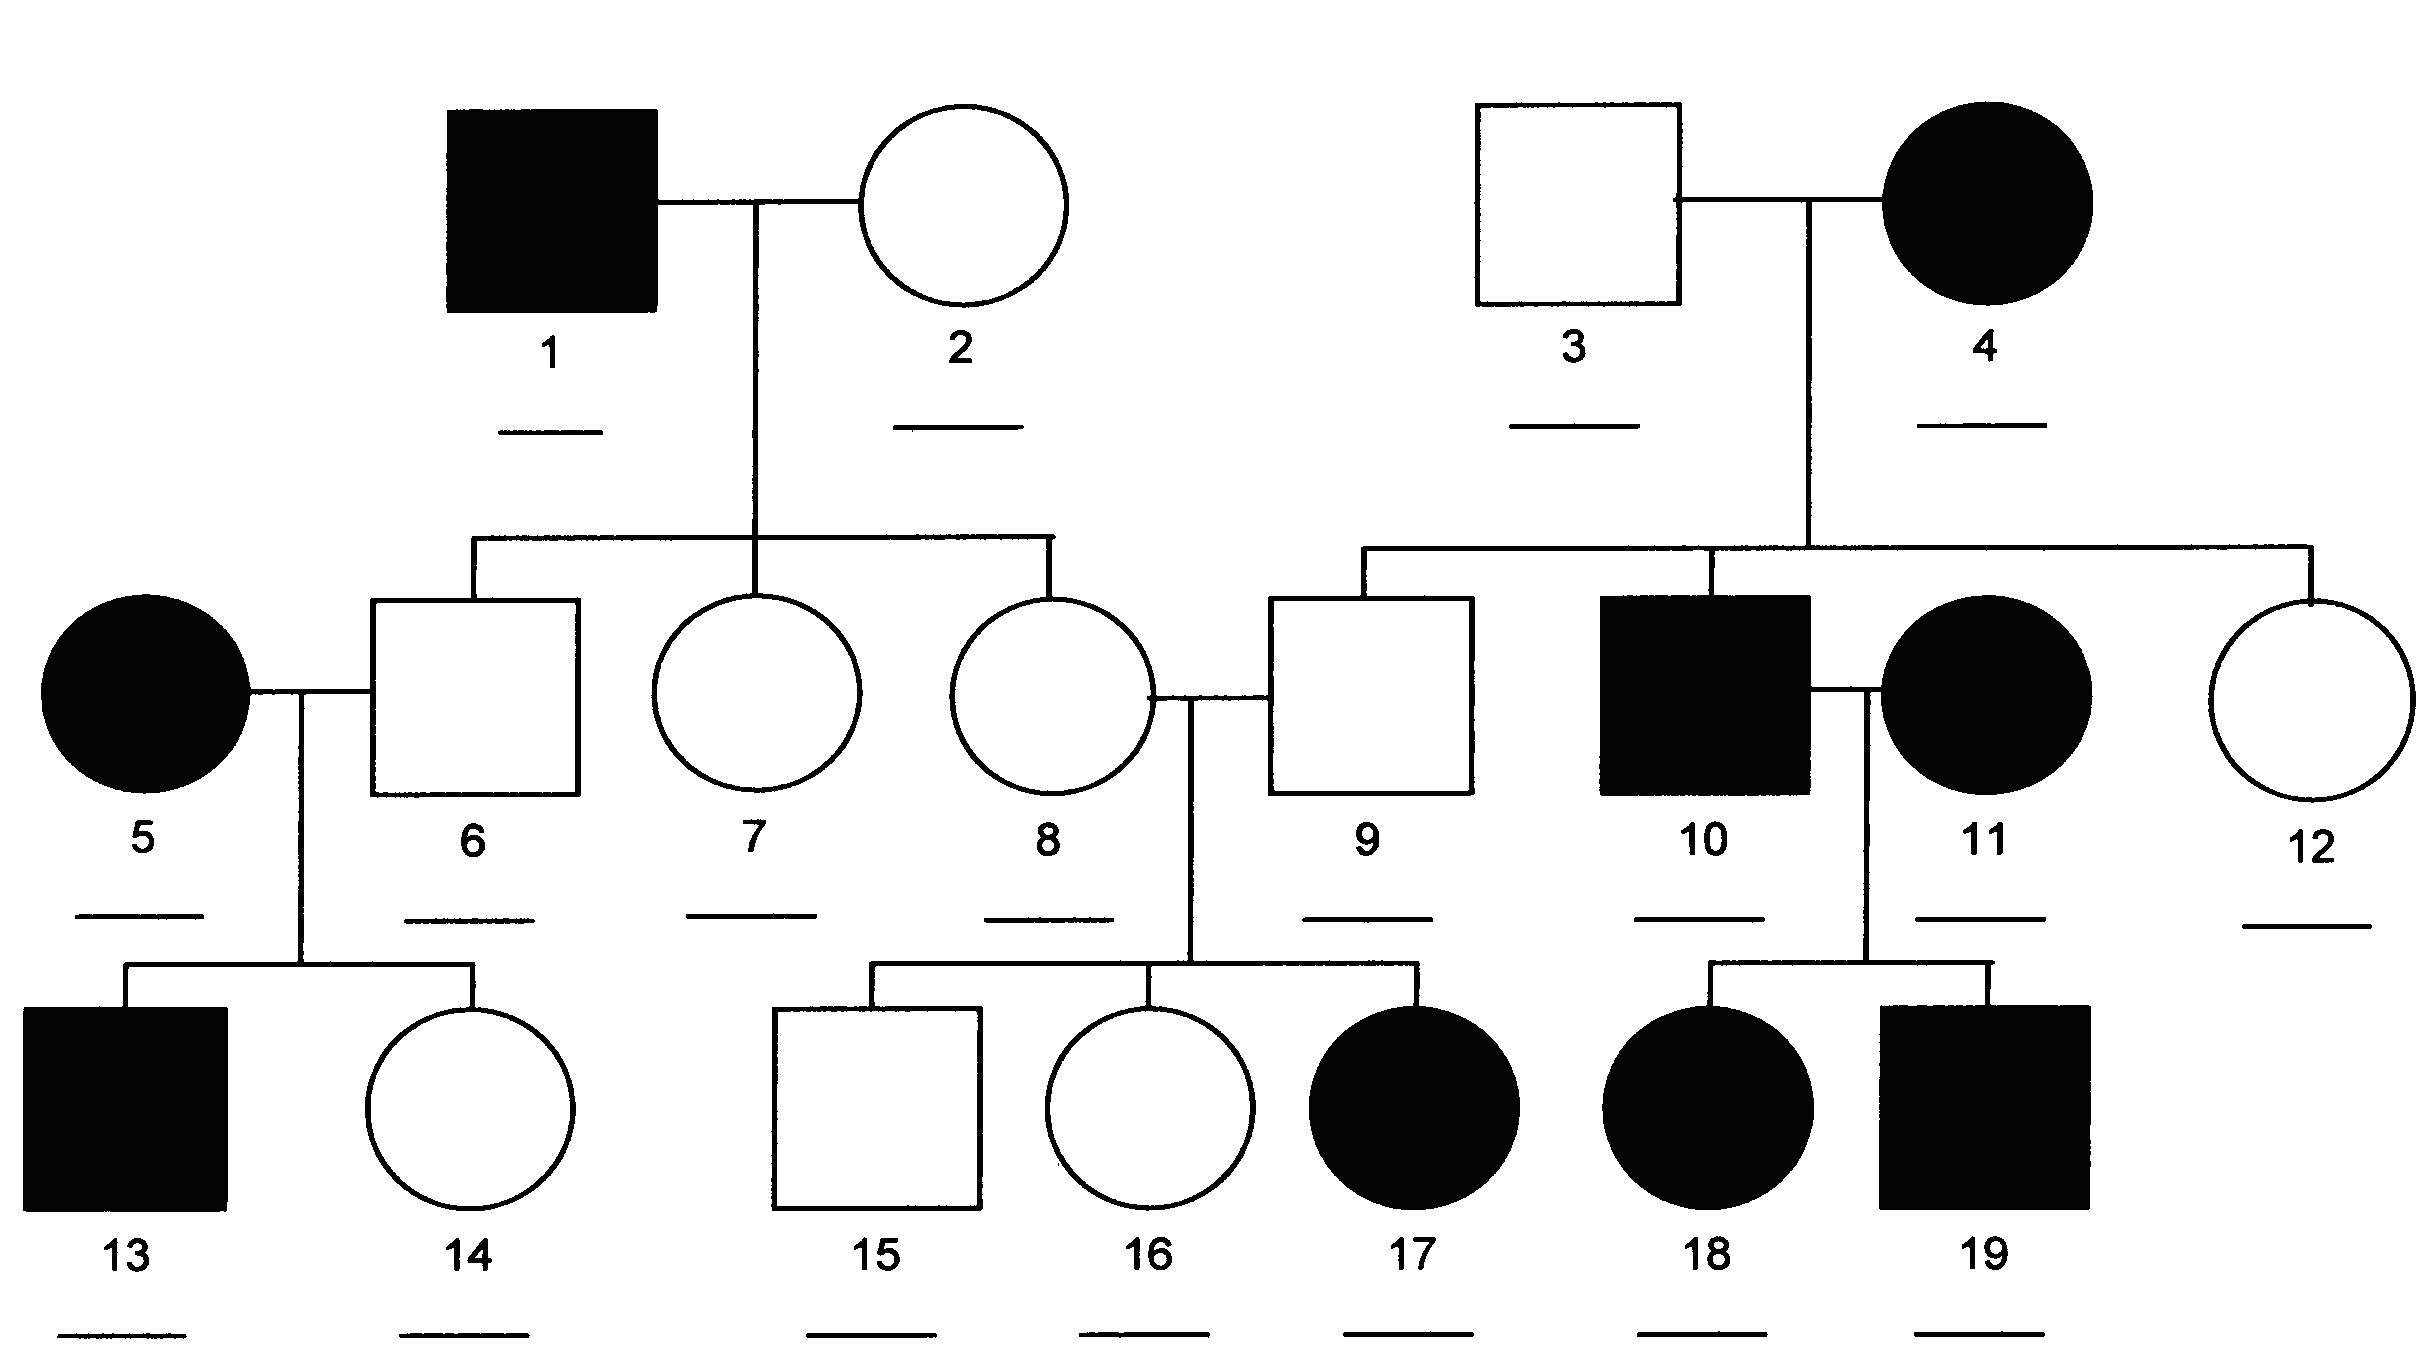
\includegraphics[width=120px]{pset1recessive.png}
\end{figure}

\item \textbf{(0.25 points)} What modes of inheritance are consistent with the following pedigree? Name an example human condition that follows this mode of inheritance.

\begin{figure}[h!]
\centering
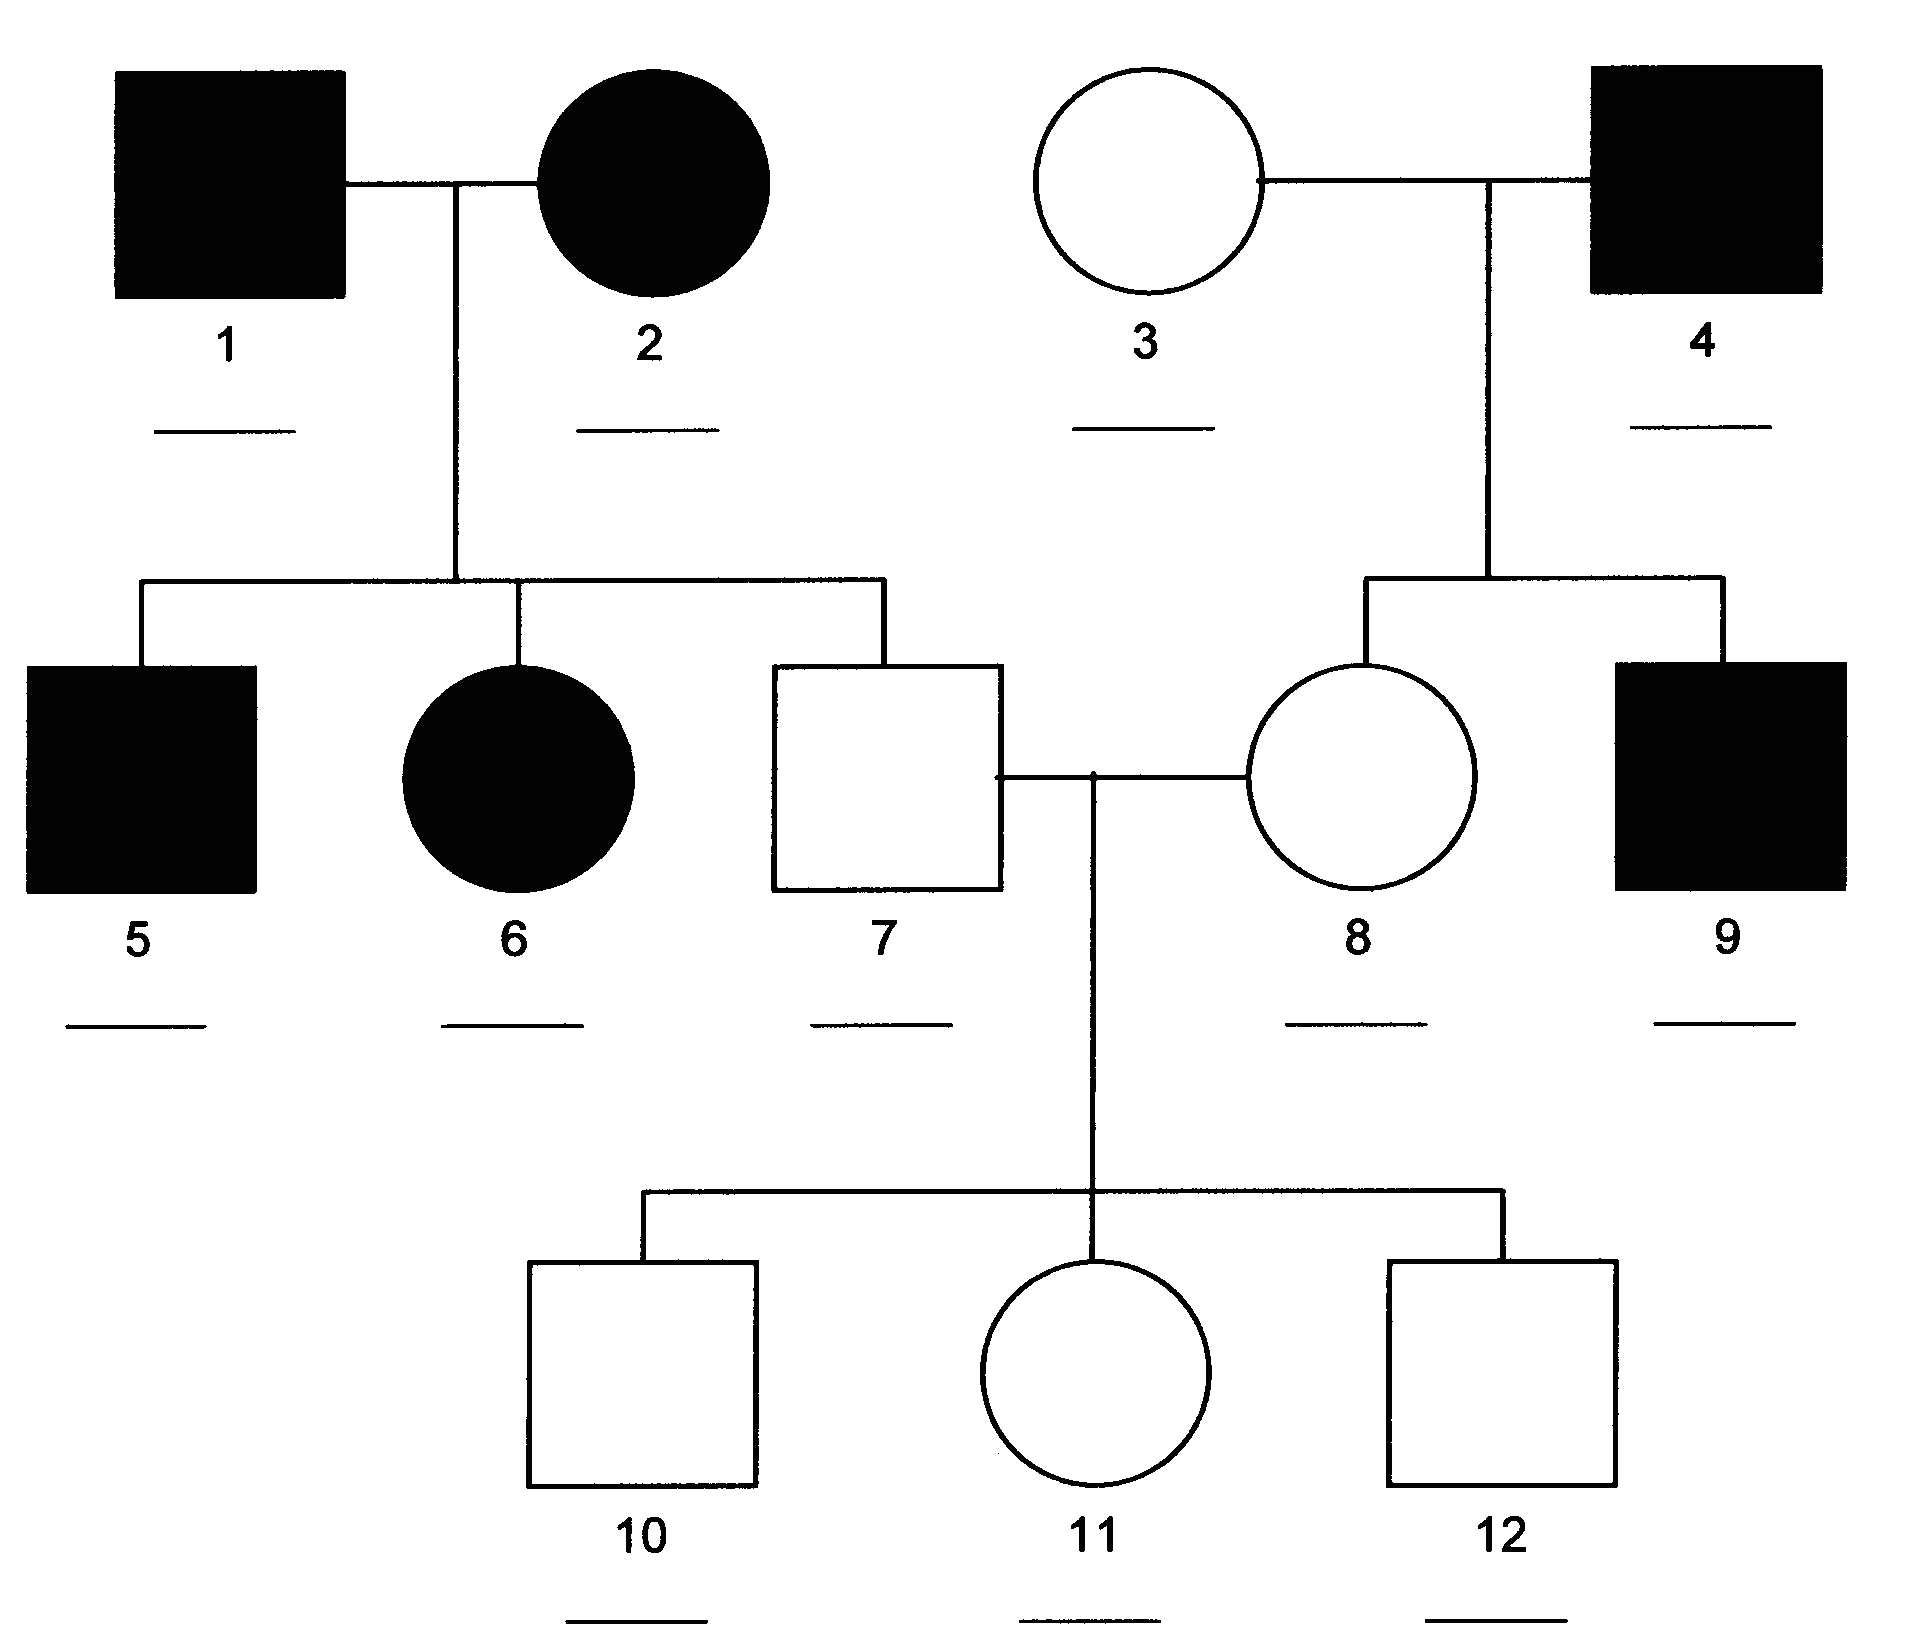
\includegraphics[width=100px]{pset1dominant.png}
\end{figure}

\pagebreak

\item \textbf{(1 point)} Navigate to \href{https://gymreklab.github.io/teaching/personal\_genomics/ps1\_resources.html}{PS1 resources} on the course website, which describes where you can find data files on the comet cluster. First, we'll get familiar with the VCF file format. For full details of VCF format, see \href{https://samtools.github.io/hts-specs/VCFv4.2.pdf}{here}. Copy the file \textcolor{purple}{pset1\_1000Genomes\_chr16.vcf} to your own directory (it is small).
\begin{itemize}
\item Lines at the top of the file marked with ``\#\#'' indicate the header. What build of the human reference genome is used in this file?
\item Look at the first entry (16:31002227). What is the reference allele? What is the alternate allele? What is the rsid?
\item What is HG00099's genotype at this position (CC, CA, or AA?).
\end{itemize}

\item \textbf{(1 point)} Individual HG00097 comes to the hospital with a blood clot. The doctor would like to treat the patient with warfarin, but is trying to figure out the correct dose. Studies have shown that \href{https://www.snpedia.com/index.php/Rs8050894}{SNP rs8050894 is associated with warfarin dosage}. Individuals with genotypes CC, CG, and GG are recommended to get 2.5, 5, and 6.5 mg/day respectively. We would like to determine the correct dose for our patient.

VCF genomes can be quite large (the VCF file for the ExAC dataset is more than 1TB!). If we want to query a specific location of the genome, it would be inefficient to scan the entire file. \textcolor{purple}{tabix} offers utilities to build an index for VCF (and other) files to enable quick access to a specific location. Use the tabix utility to index the VCF file with the following commands:
\begin{Verbatim}[commandchars=\\\{\}]
\color{purple} bgzip pset1\_1000Genomes\_chr16.vcf
\color{purple} tabix -p vcf pset1\_1000Genomes\_chr16.vcf.gz
\end{Verbatim}

Now, use the tabix utility to pull out our SNP of interest:
\begin{Verbatim}[commandchars=\\\{\}]
\color{purple} tabix --print-header pset1\_1000Genomes\_chr16.vcf.gz 16:31104509-31104510
\end{Verbatim}

What dose should the doctor give to HG00097? What about HG00099 and HG00103?

\item \textbf{(1 point)} The doctor now wonders whether HG00097 has other variants in \emph{VKOR1C}. We would like to determine whether the individual has any mutations in the protein-coding sequence of this gene. Luckily, we have a file VKORC1\_exons\_NM\_001311311.bed listing the genomic coordinates of each exon. This is an example of a BED file, which gives the chromosome, start coordinate, and end coordinate of each interval.

Intersecting genomic intervals is an extremely common task. \textcolor{purple}{bedtools} contains many utilities for working with BED files. Use the \textcolor{purple}{intersectBed} utility to look at all positions falling within the given intervals.
\begin{Verbatim}[commandchars=\\\{\}]
\color{purple} intersectBed -a pset1_1000Genomes_chr16.vcf.gz -b VKORC1\_exons_NM\_001311311.bed
\end{Verbatim}
(You'll have to edit the above to include full paths to the VCF and BED file). Does HG00097 have any variants from the reference genome in exons of VKOR1C?
% 16	31102321	rs7294 1|0

\end{enumerate}

\end{document}